\documentclass[12pt]{article}
\usepackage{geometry} % see geometry.pdf on how to lay out the page. There's lots.
\usepackage{hyperref}
\usepackage{graphicx}
\usepackage{gensymb}
\usepackage[affil-it]{authblk}
\usepackage[toc,page]{appendix}
\usepackage{pifont}
\usepackage{amsmath}

\geometry{letter} % or letter or a5paper or ... etc
% \geometry{landscape} % rotated page geometry

% See the ``Article customise'' template for come common customisations

\title{Gluss = Slug + Truss}
\author{Robert L. Read
  \thanks{read.robert@gmail.com}
}
\affil{Founder, Public Invention, an educational non-profit.}


\date{\today}

%%% BEGIN DOCUMENT
\begin{document}

\maketitle

%%% Probably will want to remvoe this as the article will not be that long

\tableofcontents

\section{Introduction}

\subsection{Motivation}

Imagine a strong, light, metamorphic robotic substance.
The uses of such a substance are limited only by our ability to imagine them.

Imagine a bridge that crawls into place in a matter of hours.
Imagine constructing a temporary highway overpass in 24 hours, or a pedestrian bridge for a festival
in the morning that comes down in the evening.

Imagine a snake-like robot that can crawl into a collapsed building and hold the roof up
while survivors are extracted.
Imagine material that combines the functionality of forklift, a crane, a bulldozer and a backhoe,
all in one machine. Imagine a very small gluss that crawl into and holds shut a wound,
temporarily taking the place of missing tissue.

\subsection{Concept: Gluss = Slug + Truss}

Imagine a metamorphic machine that forcefully assumes a variety of shapes. It moves like a mollusc or amoeba,
oozing into position as commanded. It is technically a ``machine'' because it can exert force reliably, but
it may be thought of as a material, because unlike most robots its compoents are not differentiated.

Although someday an actual chemical substance may do this, today it can be constructed from commercial components
and 3D-printable parts. This paper introduces the \emph{gluss} approach to building metamorphic dynamic robots
and static machines.\footnote{ ``Gluss'' is a portmaneau of ``Slug'' and ``Truss'' because we are attempting to
build a truss, or space frame, that is capable of moving like a slug, or octopus if you prefer.
The word \textit{gluss}
should be used as a substantive noun in English, much like the word \textit{clay} is used.
The use of \textit{glusses} the plural
of \textit{gluss} should be rare and refer to different kinds of metamorphic material, such as the expression
``four clays'' suggests four distinct types of clay without specifying how many kilograms of each one means.}

Massively scalable robots have often been proposed. Our particular approach is to use linear actuators,
which are rod-like machines that can make themselves shorter or longer. These are tied together using
a relatively new joint \cite{song2003spherical} which allows, for example, as many as 12, but more realistically 4,
members to be joined together sturdily at a single point.
A 3-D printed embodiment presented here and called the \emph{turret joint} to allow the
change of angle to allow gluss to ooze about. Some gluss consists of some actuators joined together
with some turret joints and whatever batteries and control microelectronics are needed. In the
working, crawling robot discussed here, the \emph{3TetGlussBot}, there are two controllers and two batteries
in addition to the 12 actuators and the 6 multi-member turret joints, but 3TetGlussBot is only
a small amount of the gluss we hope to build.

\begin{figure}[!ht]
  \centering
    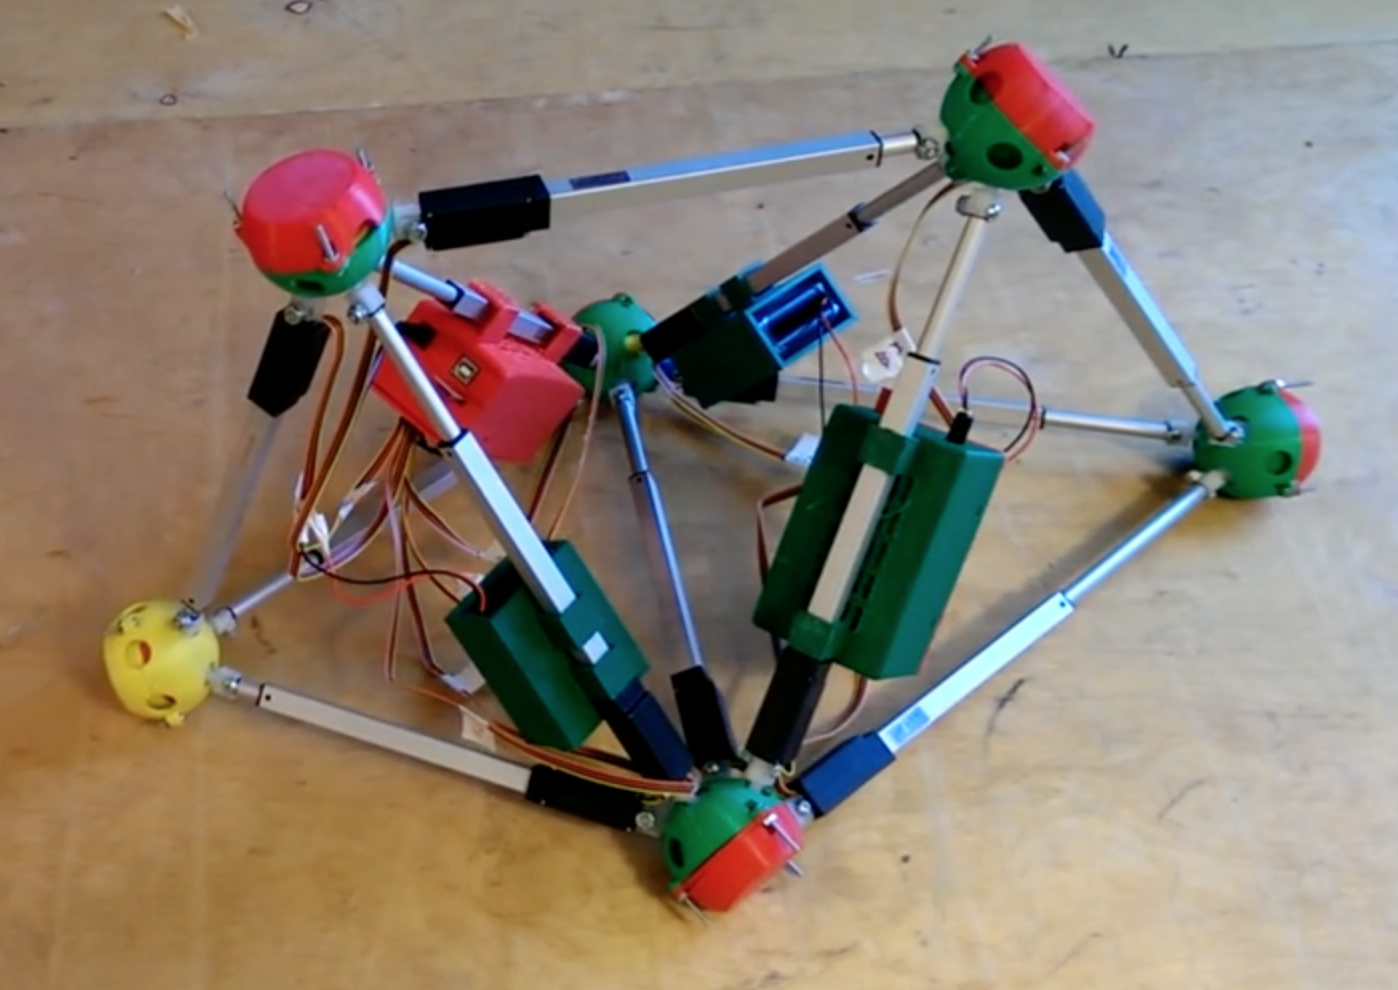
\includegraphics[width=0.5\textwidth]{3TetGlussBotPhoto.png}
    \caption[3TetGlussBot Photo]{Photo of the 3TetGlussBot.}
      \label{3TetGlussBotPhoto}
\end{figure}


We present two geometries for gluss which have the advantage of being regular, thus allowing us to
seamlessly connect any number of actuators into any amount of gluss.
The specific actuators, their 12 Volt power supply, control via Arduino Mega microcontrollers, and
coordination via BlueTooh from an Emacs E-LISP control program are discussed.

\section{The \textit{Turret Joint}}

\subsection{The Need}

The way to make some thing large, light, and strong is to make it inherently rigid by building it
out of triangles. In a single plane, this is called a \emph{truss} \cite{ambrose1993building}, and more generally is called
a \emph{space frame}.  Space frames made completely from triangles tend to be rigid even if the
joints that connect members are allow motion, such as a pin joint or a ball-and-socket joint. This
is an advantage because strain (that is, a slight change in the geometry of the frame) cannot cause
the joint to fail, as it can with a welded joint.

But we seek a space frame that can change its shape dramatically. Imagine a radio tower in which
each girder has been replaced with an actuator that can get longer or shorter. Such a tower could
bend its top down to the ground, or event
tie itself into a knot. To accomplish this, the joints must support significant although not
limitless range of motion. 

The spherical joint inveted by Song, Kwon and Kim \cite{song2003spherical} is such a joint.
We name this joint the \emph{Turret joint}.
In the embodiment mentioned here joint presented here supports somewhat less than a theoretical
$36\degree$ of motion.
When properly configured to support the regulat nets of actuators we propose,
it allows the gluss to be a moving spaceframe. It happens that the specific actuators we use
are geared such that they hold their position forcefully without power, so the resulting gluss
can move into position and then be powered off to be a temporarily static space frame.

One could also use this joint with members which are not actuators. For example, we first
constructed the joint with carbon fiber rods. In essence it is then becomes a construction with continuously
variable member lengths liberated from using a finite set of angles.

\subsection{Geometry}

\begin{figure}[!ht]
  \centering
    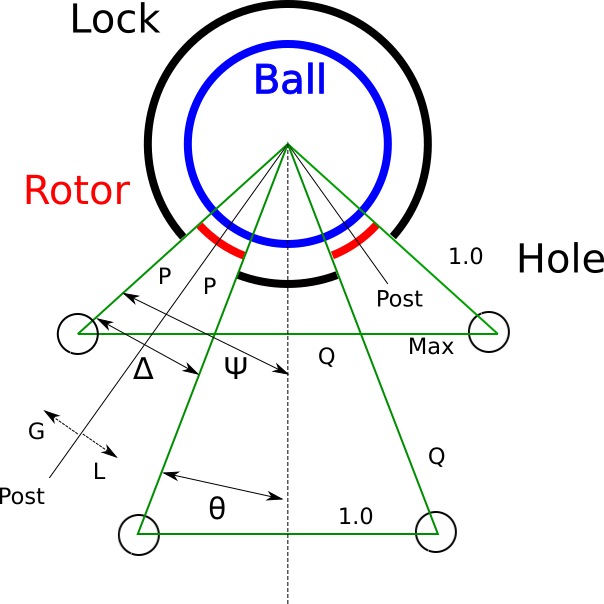
\includegraphics[width=0.5\textwidth]{ConstraintDrawing.png}
    \caption[Constraints]{Turret Joint Geometry Constraints}
      \label{constraint-drawing}
\end{figure}

%% \begin{figure}[!ht]
%%   \centering
%%     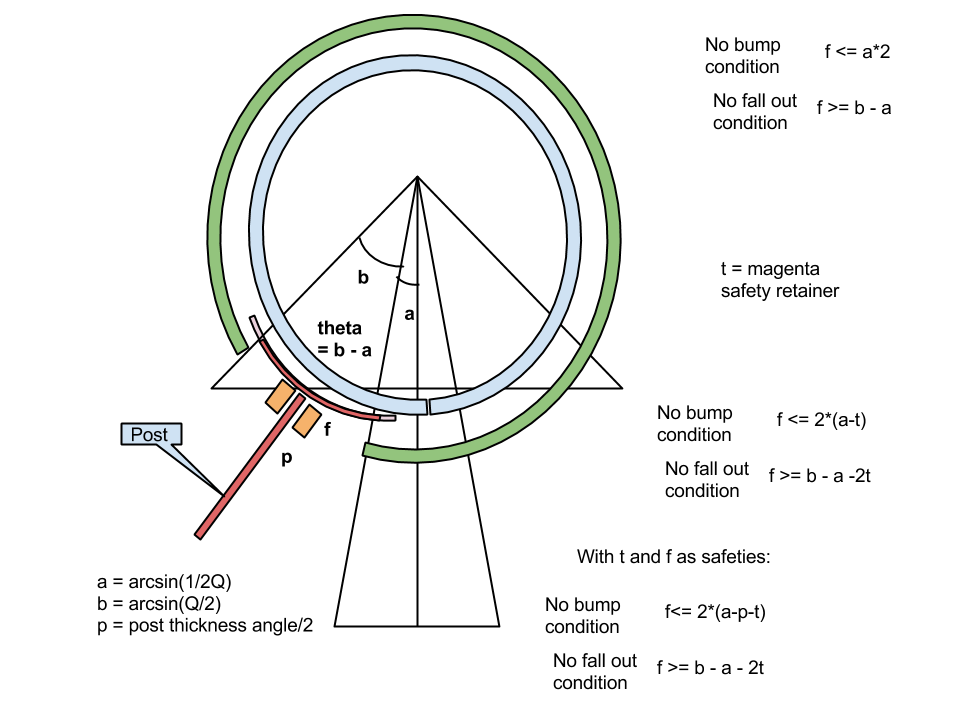
\includegraphics[width=0.5\textwidth]{TurretJointMath.png}
%%     \caption[TurretJointMath]{The Turret Joint analyzing the range of motion. TODO: This needs to be improved, showing the golden triangle and golden gnomon!}
%%       \label{TurretJointMath}
%% \end{figure}

How versatile can we make the turret joint?

In particular, since we are attempting to build gluss which is regular in its use of actuators, we may ask:
What is the maximum range of motion in our
actuators which we can usefully employ in our gluss?
To work independent of scale, we use the symbol $Q$ to denote the ratio of the actuator at its
longest to its length at its shortest.
The particular actuators we use have a $Q$ of 1.5. But is that the maximum $Q$ that we could utilize? Or is
it already too high?

One way to approaoch this problem is to consider a single triangle formed by joints and actuators.
The joint must support the most acute triangle
that can be formed with the three acutators and the most obtuse triangle that can be formed with the actuators.

In fact it is a surprising result that we prove in Appendix \ref{phiproof} that the maximum $Q$ which can be utlized
by an ideal turret joint happens to be
the famous golden ratio, $\varphi$, and the maximum deviation for any one member coming
into the joint is $36\degree$.
Thus in Figure \ref{constraint-drawing} the triangles drawn are in fact a Golden Triangle and a Golden Gnomon.
This is interesting but has little to
do with a real-world joint, which will support less variation because the ``post'' must have a
certain thickness and the ``rotor'' must have a lip
slightly larger than the hole in order to remain locked in place.
Furthermore, the joint adds a certain necessary thickness, the minimum length
 from joint-center to joint-center will be somewhat greater than from actuator tip to actuator tip.

 However, the theoretic result is a valuable guideline and makes a $Q$ for a physical actuator of 1.5 seem quite appropriate.

 \subsection{Embodiment}

 Although the joint could be machined or formed in some other way,
 3D Printers have made the construction of the Turret Joint far easier.
 We have designed a complete set of components needed to 3D print the joint and the rotors to attach to
 the linear actuators. These models are created with OpenSCAD, a functional parametric modeling program.

 Our experience has been that the common plastics PLA and ABS are adequate for the Turret Joint,
 but have found that nylon, which is far tougher and less prone to cracking, is superior for the
 rotors which bolt directly to the actuators.

\subsection{Geometries Specific to Gluss}

Although the possibly ways to configure acutators and joints is limitless, the simplest thing is to
use regular, repeatable geometries. The two most obvious are the Boerdijk–Coxeter helix
(more easily called the \textit{tetrahelix})
\url{https://en.wikipedia.org/wiki/Boerdijk%E2%80%93Coxeter_helix}
    (See Figure \ref{Boerdijk-Coxeter-Helix}) and the \emph{Octet Truss}
    \cite{richard1961synergetic} (See Figure \ref{octet-truss-patent}).
    
Roughly speaking, the Tetrahelix is a good way to make a long shaft or tentacle, and the octet truss
is a good way to make a planar shape. The purpose of a tentacle is to curl, and the we have no word for
a plane that roll itself up into a cylinder or cone or form a barrel vault. Buckminster Fuller discusses
both the tetrahexlix and octet-truss \cite{fuller1982synergetics} in terms of static structures and geometries.

\begin{figure}[!ht]
  \centering
    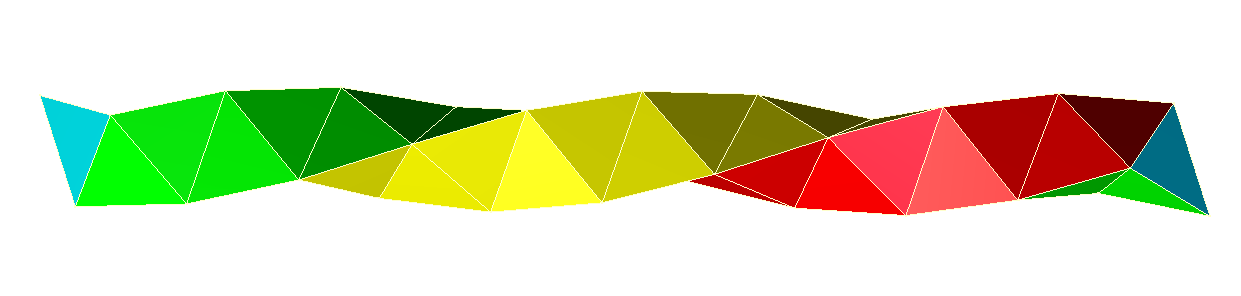
\includegraphics[width=0.5\textwidth]{Coxeter_helix_3_colors_cw.png}
    \caption[Boerdijk–Coxeter Helix]{Boerdijk–Coxeter Helix, or Tetrahelix, By Tomruen (Own work)
      [CC BY-SA 4.0 (\href{http://creativecommons.org/licenses/by-sa/4.0}{http://creativecommons.org/licenses/by-sa/4.0})], via Wikimedia Commons}
      \label{Boerdijk-Coxeter-Helix}
\end{figure}

\begin{figure}[!ht]
  \centering
    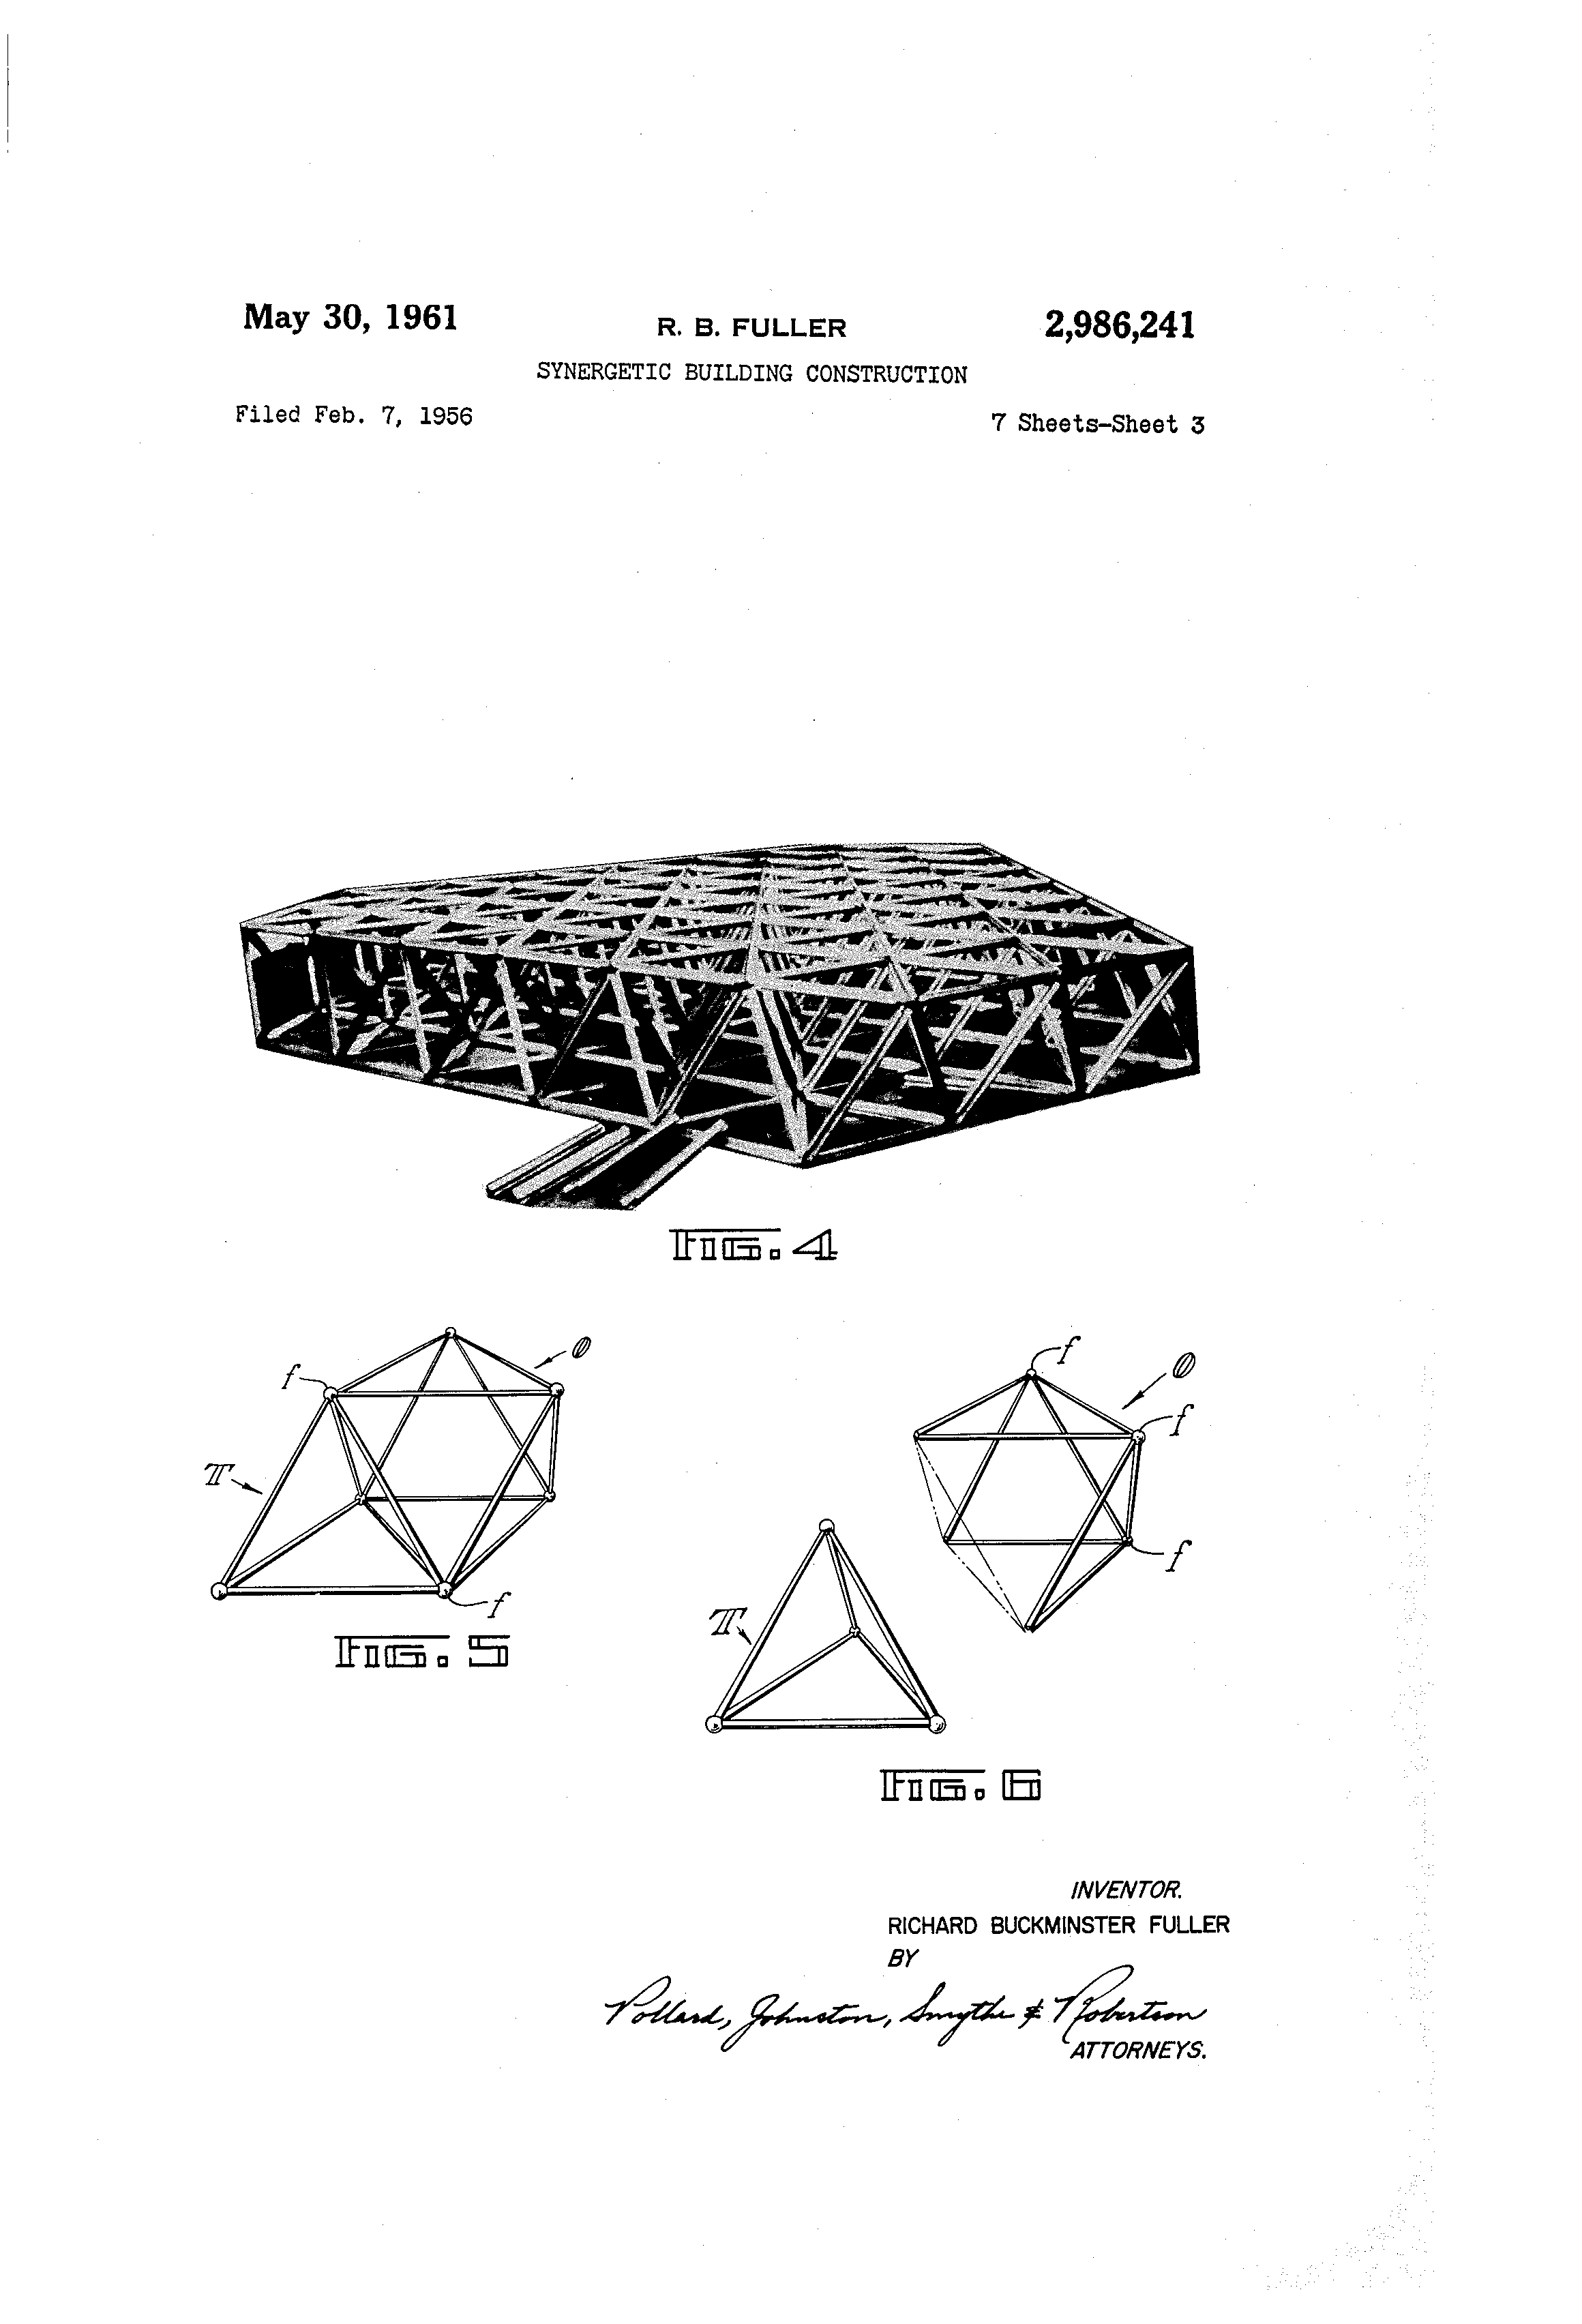
\includegraphics[width=0.5\textwidth]{US2986241-2.png}
    \caption[The Octet Truss]{The Octet Truss, from Buckminster Fuller's patent.}
      \label{octet-truss-patent}
\end{figure}

The Octet Truss reflects the geomtry called the ``cuboctahedron.''

Because the Turret Joint does not support infinte revolution of all members, the joint, or the ``lock'' or ``stator'' in particular,
must be adjusted to the regular geometry that one is implementing.  The Figure \ref{lockcomparison} indicates this difference.
The image is from TurrentJoint.scad
\href{https://github.com/PubInv/turret-joint/blob/master/Models/TurretJoint.scad}{https://github.com/PubInv/turret-joint/blob/master/Models/TurretJoint.scad}, an
open-source file that can be used to 3D print all of the turret joint components. It shows a lock part for the Tetrahelix geometry
on the left, and the more expansive Octet Truss geometry on the right. Observe that some of the holes are half in this part,
and have in the ``cap'' parts not shown here.

\begin{figure}[!ht]
  \centering
    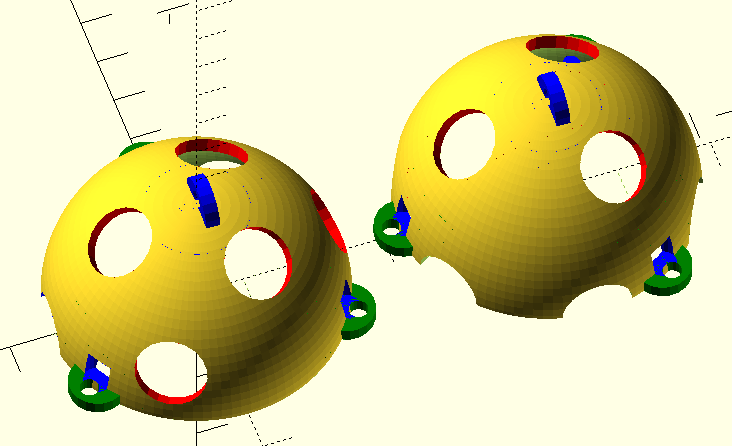
\includegraphics[width=0.5\textwidth]{TetrahelixLockVsOctetTrussLock.png}
    \caption[Lock Comparison]{Lock Comparison}
      \label{lockcomparison}
\end{figure}


At some point the glussbot will bump into itself.

\subsection{Range of Motion for Actuator Nets}

The result that in theory a perfect joint supports a $Q$ of approximately $1.618$ does not imply that any actuator net can acheive any
geometry. 

An interesting question is:

In a tetrahelix formed of actuators with a given $Q$, how many cells (tetrahedra) are required for the glussbot tip to touch itself?
In other words, if a tetrahelix tentacle is bolted to the ground, how many cells are required for the tip to reach the ground?
Or the even greater challenge, to touch the base of the tentacle itself?

More matehmatically, can we define a ``radius of curvature'' as a function of $Q$ for a tetrahelix?

For the Octet Truss architecture, it would be nice to know a radius of curvature that supports forming a cylinder. Would this
be isotropic in direction, or would it be strongly anisotropic?  

\section{Linear Actuators}

We use the term Linear Actuator to refer to any device that is capable of changing its length. When
used in gluss it might be called a \emph{glussion}, a single particle of gluss. Our current gluss
uses a commercial linear actuator (the Firgelli L-16-140-35-12-P,
\href{http://www.firgelli.com/L16_Linear_Actuators_p/l16-p.htm}{http://www.firgelli.com/L16\_Linear\_Actuators\_p/l16-p.htm}
)
that costs about \$80 and exerts about 50 Newtons of force.
Turret joints that are 3D printed in ABS plastic have been strong enough for this level of force.

However, in principle there is not reason we could not use the enormous hydraulic cylinders
used backhoes, bulldozers, and other earth moving equipment. These would of course require much
stronger joints, probably not made out of plastic.

We could also attempt to make smaller actuators, to make a pocket-sized gluss. This is probably
a greater technical challenge, because it is relatively difficult to make small electric motors.

The current actuators use a rotary motor with a lead screw. This has the advantage of great
strength relative to their size, and the retaining position forcefully. It has the disadvantage
of being relatively slow. It would be interesitng to build a gluss out of linear motors, for
example tubular linear synchronous motors. These would be much faster than the lead-screw type
actuators, resulting in a much faster gluss. 

\section{Control and Motion}
\subsection{Architecture of the 3TetGlussBot}

We have constructed the simplest possible Tetrahelix-based glussbot that is capable of locomotion.
It comprises:
\begin{itemize}  
\item 12 actuators
\item 6 turret joints
\item 2 12V battery packs
\item 2 controller units, each of which comprises:
\begin{itemize}  
\item 1 Arduino Mega microcontroller,
\item 1 custom Arduino Mega shield hosting 6 1-amp motor channels and a BlueTooth module,
\end{itemize}  
\end{itemize}

\begin{figure}[!ht]
  \centering
    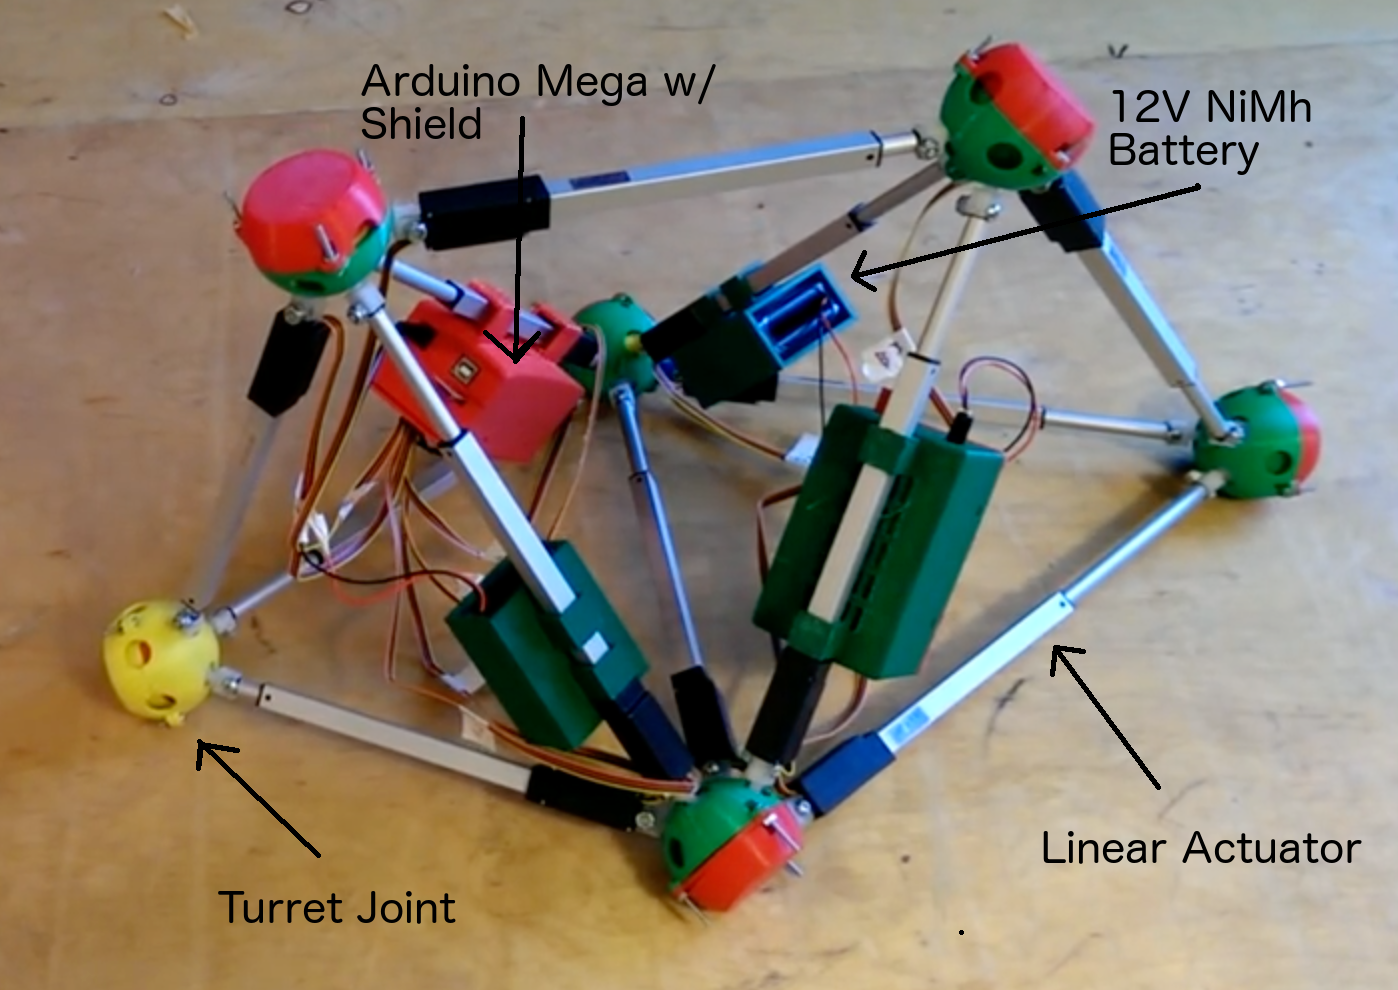
\includegraphics[width=0.8\textwidth]{3TetGlussBotPhotoAnnotated.png}
    \caption[3TetGlussBot Components]{3TetGlussBot Components}
      \label{annotated}
\end{figure}


Each controller module electrical system can support up to 6 actuators, so two are required for the 3TetGlussBot.
The BlueTooth modules open serial connections controlled by a computer.
The Arduino Mega is programmed to support commands addressed to each or all of the actuators, and
to provide feedback. The comptuer and the Arduino control programs communicate via S-Expressions
implemented with our own module. This is very analagous to sending JSON back and forth.

Commands to and feedback from the controller modules are managed by an Emacs E-Lisp program.
This program organizes motion into ``poses''. A serious of poses make a dance.
In order to dance, the program must synchronize the completion of poses, because there is no
guarantee how long it will take to achieve a pose. The time to reach a position in theory
depends on the voltage level provided by the battery and the force resisting the motion.
In practice, when lightly loaded by moving only itself, the time is relatively predictable. It takes
about 2 seconds for the 3TetGlussBot to go from its most compact state to its largest, most expanded state.

\subsection{Open Source Realizations}

We have provided everything necessary to construct gluss in the form of FLOSS. Providing an ``Instructable''-style
how-to guide is beyond the scope of this article, but a semi-skilled electronics hobbyist can use the
following resources to construct their own GlussBot.

\begin{description}
  
\item [Turret Joint]
  The Turret Joint is implemented via OpenSCAD files. The file itself is here:
  \href{https://github.com/PubInv/turret-joint/blob/master/Models/TurretJoint.scad}
       {https://github.com/PubInv/turret-joint/blob/master/Models/TurretJoint.scad}.
       The model may be observed without even installing OpenSCAD, and even 3D printed,
       from the same file using the customizer feature of Thingiverse.
       \href{http://www.thingiverse.com/thing:1043716"}{http://www.thingiverse.com/thing:1043716"}
  \begin{figure}[!ht]
    \centering
    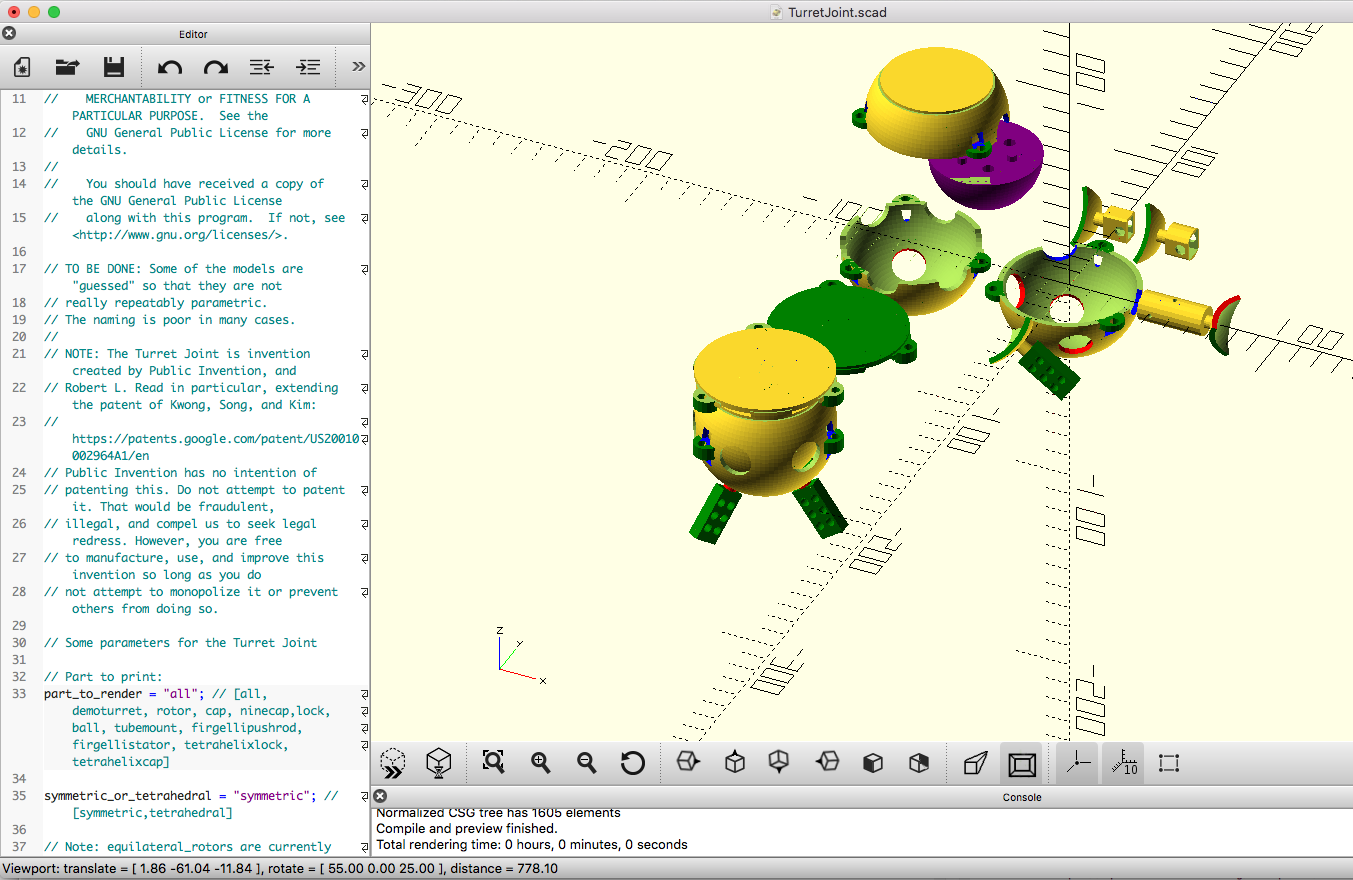
\includegraphics[width=0.5\textwidth]{OpenSCADScreen.png}
    \caption{OpenSCAD Screen shot}
  \end{figure}
  
\item [Robot Controller Shield]
  An Arudino Mega Shield may be ordered directly from OshPark, where it is titled the \emph{3x2 Motor Controller MegaShield, v0.2}.
  The \href{https://oshpark.com/shared_projects/fijpozoB}{https://oshpark.com/shared\_projects/fijpozoB} shield
  may be useful to anyone who wants to control up to six DC motors (up to 1 amp each) at the same time, via Bluetooth.
  Alternatively, you may use the Eagle Soft CAD files, which can be found here:
  \href{https://github.com/PubInv/gluss/tree/master/GlussPCBv0.1}
  {https://github.com/PubInv/gluss/tree/master/GlussPCBv0.1}
  \begin{figure}[!ht]
    \centering
    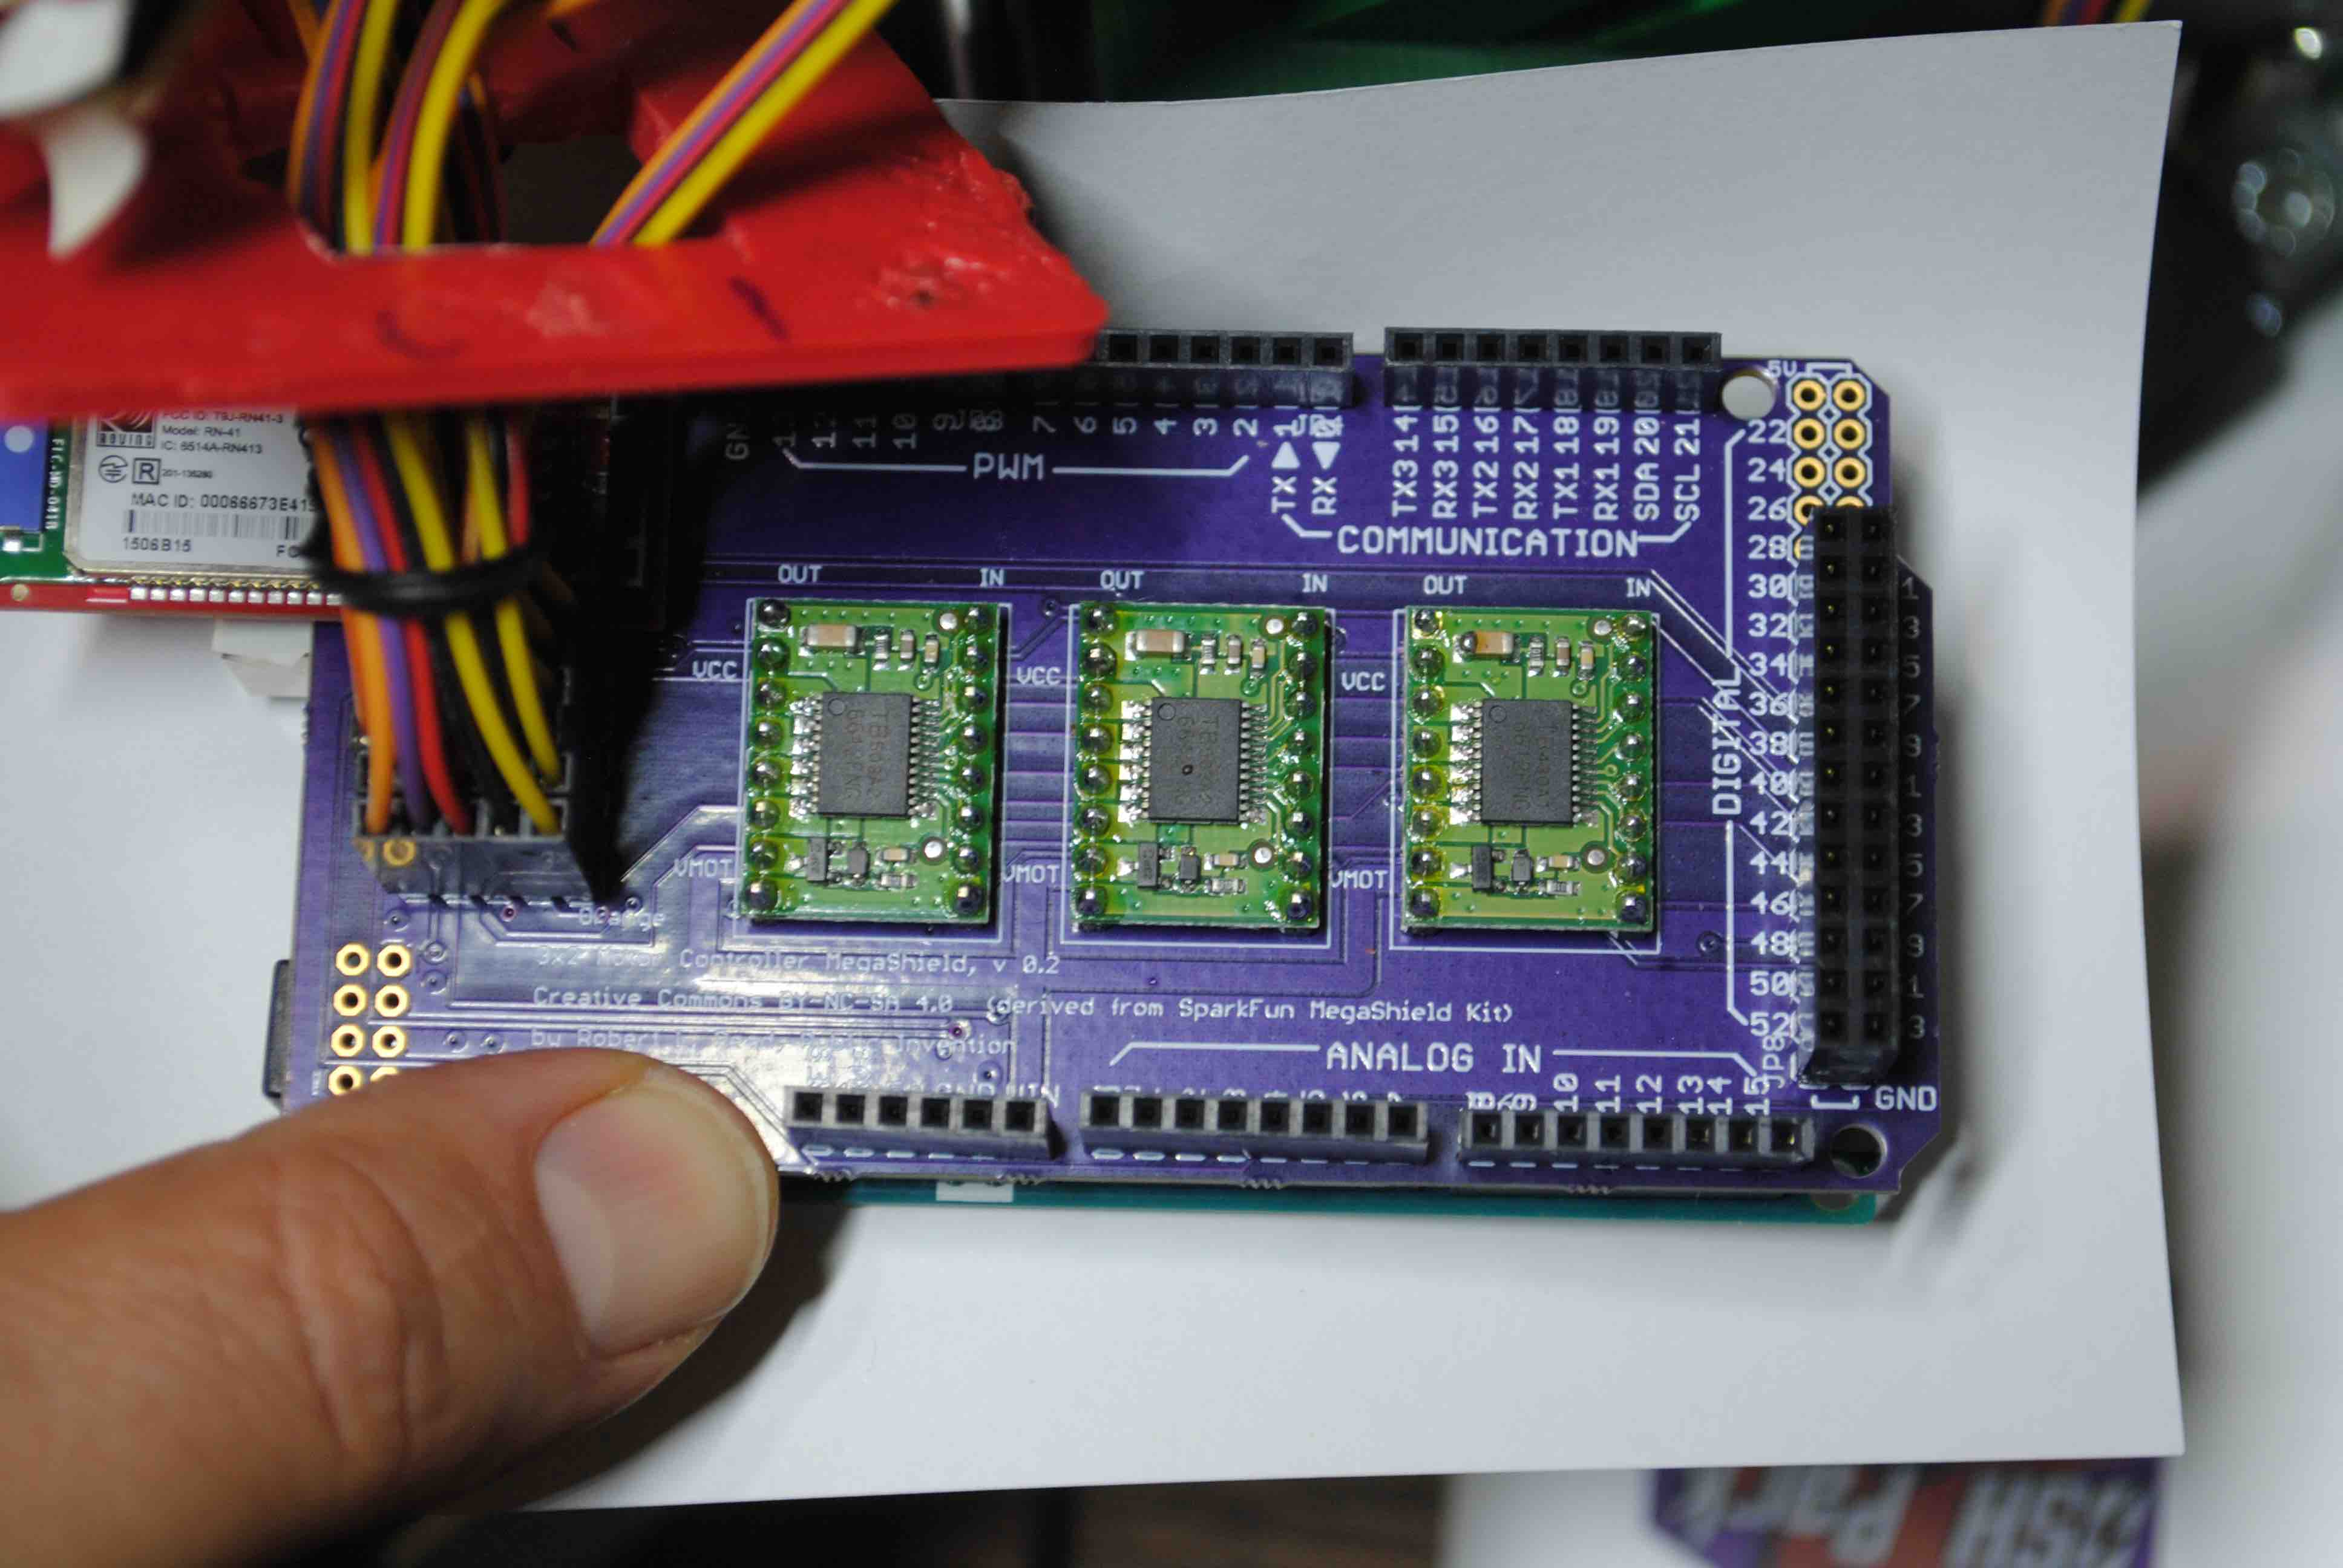
\includegraphics[width=0.5\textwidth]{MotorControllerInPlace.JPG}
    \caption{Arduino Mega Shield board}
  \end{figure}

\item [Control Software]
An Emacs LISP program which controls the 3TetGlussBot via a command-line interface:
\href{https://github.com/PubInv/gluss/blob/master/emacs-ctl.el}{https://github.com/PubInv/gluss/blob/master/emacs-ctl.el}

An Arduino Sketch which implements a device driver for the GlussBot Controller Shield is required as well:

\href{https://github.com/PubInv/gluss/blob/master/GlussPCBv0.1/GlussPCBv0.1.ino}
     {https://github.com/PubInv/gluss/blob/master/GlussPCBv0.1/GlussPCBv0.1.ino}.
     This sketch needs the Arduino module S-Expr.
     
\item [S-Expr]
  The \href{https://github.com/PubInv/S-Expr}{https://github.com/PubInv/S-Expr} Arduino S-Expr project and its
  \href{https://github.com/PubInv/Arduino-S-Expr-Test}{https://github.com/PubInv/Arduino-S-Expr-Test} test project
  may be useful to anyone who wants to control an Arduino from Lisp or prefer S-Expressions to the closely related JSON format.

  
\end{description}

\subsection{Speed Performance}

The 3TetGlussBot is capable of ``walking'' and turning. Some might prefer the term ``crawl'' to ``walk'' in
this case. It can move forward awkwardly at a rate
of about five inches per minute. It can turn 30 degrees in about 20 seconds [TODO -- need to check this.]
We intentionally chose to make the simplest amount of gluss that we thought would be capable of locomtion.
We believe that by adding more gluss, that is, by connectiong more tetrahedra in the tetrahelix,
we will open new and more efficient locomotion gaits.

The present mode of walking avoids dragging the pseudopods by leaning to one side or front or back and
then lifting the pseudopod, moving it forward (without ground contact), and placing it down again.
Such a gait may be able to handle rugose terrain better than a gait that drags feet.

The current programmed gaits are probably not optimal.
We have programmed locomotion of the 3TetGlussBot only to prove that it can be done, not to make
a performant robot.


\section{Future Steps}

Actions are available at the research level and at the hobbyist level, and we refuse to draw
a crisp distinction betwen the two, but we have organized these from most difficult to least
difficult.

\begin{description}
\item [Remove Scale:] At present the 3TetGlussBot is programmed as specific geometry. Any program
  written for it would have zero valua for a robot of the same general shape but built with considerably
  more actuators. Ideally, we would be able to program gluss completely independent of the scale
  of implementation. We would treat it as a true metamorphic material, rather than as a net of
  actuators arranged in a particular configuration. This can be considered a problem of pure
  mathematics, touching on wavelet theory, for example. It blends into computer science and
  finally robotics.
\item [Math of Ideal Systems:] What configurations are possible of ideal and real-world gluss?
  For example, what is the maximum radius of curvature of an octet truss employing joints
  and actuators of specific properties? This is primarily in the realm of geometry, and perhaps
  computational geometry.
\item [Force Performance:]
It would be be nice to answer the questions such as:
\begin{itemize}  
\item If a 5-tetrahedron tetrahelix were bolted to a frame and extended horizontally, how much
  weight can it support at the free end?
\item If a gluss bot crawled under a car and sought to jack up the car enough for a tire
  to be changed, how forceful would each actuator have to be?
\item If a large glussbot crawled across a chasm, could a truck or a human being safely move
  across it without danger of collapse?
\end{itemize}
We have not attempted to analyze gluss in terms of force performance. We believe this would
be analagous to analysis of static space frames using the dynamic configuration at a point.
Finite elment analysis is a standard approach to this.
\item [Cheap Actuator:] The gluss concepcts heightens the need for very inexpensive linear
  actuators. The current actuators at \$80 make construcitng a 100-actuator glussbot very expensive.
  It should be possible to build a linear actuator for 1/10th of this cost, although it may require
  giving up some advantages. Creating a new point in the spectrum of actuators desings would greatly
  expand the possibilities of gluss.
\item [Applications:] A killer application would help motivate the gluss concept. This does not
  require engineering, but requires careful thought.
\item [Quick Joint:] If all of the turret joints in the 3TetGlussBot are dissassembled so that
  the linear actators can be stacked together for efficient transport, it takes more than an hour
  to bolt them back together. It would be very convenient to have a joint that could be
  disassembled and assembled more quickly. We suspect that it is possible to build a magnetic
  joint similar (but larger) than those used in the GeoMag toy.
\item [Construction System:] If we imagine the members connecting the joints are not actuators but
  simply rods that can be cut to any length, we have a construction system for making spaceframes.
  Explore the possibilities of such a construction system to make organic and interesting shapes
  freed of rectilinear limits.
\item [Build Simulator:] A 3TetGlussBot can be constructed for about \$1300. Nonetheless this
  is beyond the means of many hobbyist. A simulator would allow one to research locomotion and
  motion without cost. The open-source, browser deliverable physics engine ``Cannon.js''
  provides all the basic machinery needed to build such a simulator.
\end{description}


\section{Contact and Getting Involved}

The Gluss Project \href{http://pubinv.github.io/gluss/}{http://pubinv.github.io/gluss/}
is a free-libre, open-source research, hardware, and software project that welcomes volunteers.
It is our goal to organize projects for the benefit of all humanity without seeking profit or intellectual property.
To assist, contact \href{mailto:read.robert@gmail.com}{<read.robert@gmail.com>}.

\bibliographystyle{IEEEtran}
\bibliography{IEEEabrv,gluss}

\newpage
\appendix

\label{phiproof}

\section{Maximum usable Q = $\varphi$}

Defining all angles against a center line between two rotor holes in a plane,
let:

$ A \equiv $ Min Actuator Length

$ Z \equiv $ Max Actuator Length

$ Q \equiv \frac{Z}{A} $,  The ratio of the actuator lengths, noting that $Q \geq 1$.

$ G \equiv $ Greatest Angle Reachable by Center of Rotor

$ L \equiv $ Least Angle Reachable by Center of Rotor

$ \theta \equiv $ Angle of Inmost Edge of the Rotor Hole

$ \psi \equiv $ Angle of Outmost Edge of the Rotor Hole

\begin{figure}[!ht]
  \centering
    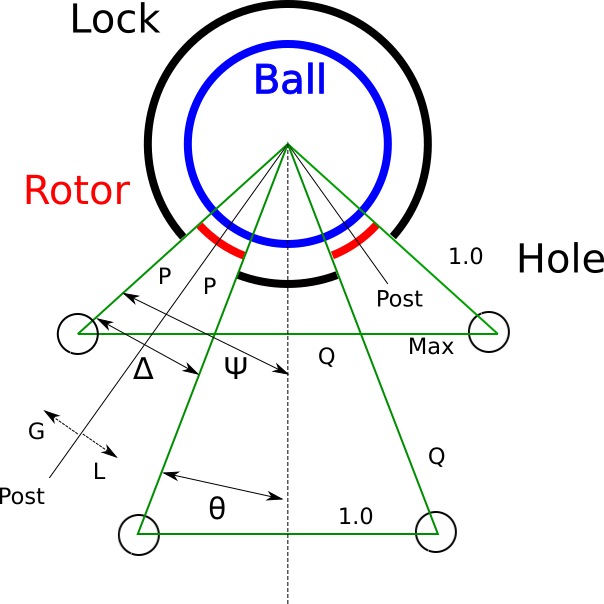
\includegraphics[width=0.5\textwidth]{ConstraintDrawing.png}
    \caption[Constraints]{Turret Joint Geometry Constraints}
      \label{constraint-drawing}
\end{figure}

\bigskip

What $\theta, \psi$ maximizes $Q$ and what is $Q$?

\bigskip

We will define the angle of the hole to be:

\[ \Delta \equiv \psi - \theta \]

From the diagram:

\[
G \equiv \arcsin{ \frac{\frac{Z}{2}}{A}} \equiv \arcsin{\frac{Q}{2}}
\]
\[
L \equiv \arcsin{ \frac{\frac{A}{2}}{Z}} \equiv \arcsin{\frac{1}{Q \cdot 2}}
\]

We then place engineering constraints upon these variables to represent physical conditions
which preclude the function of the joint.
We name these constraints \textit{meet}, \textit{bump}, \textit{capture}.

The \textit{meet} condition means that post is actually within the hole.

The \textit{bump} condition means that the rotors don't bump into each other
in their extreme position.

The \textit{capture} condition means that the the rotor can't fall out of the hole.

In both cases, we have have the capture constraint:

\[ \tag{capture} \Delta \geq G - L \]

To realize the most acute position, we have constraints:

\[ \tag{acute meet} \theta \leq L \]

\[ \tag{acute bump} \frac{\Delta}{2} \leq \theta  \]

To realize the least acute position, we have constaints:

\[ \tag{obtuse meet}  \psi \leq G \]

It is perhaps obvious that the rotors cannot bump in the most obtuse position, but we observe that:

\[ \tag{obtuse bump} 360\degree - 2\cdot \psi \geq \frac{G - L}{2} \]

is invariably true because $2\cdot\psi < 180\degree$ because psi is a half angle of a triangle, and likewise $\frac{G - L}{2} < 180\degree$.

When we attempt to set $G$ and $L$ to be as wide apart as possible by asserting $G \equiv \psi$ and $L \equiv \theta$, we must
ensure that all of thse constaints are true. The two meet conditions become true by equality. Likewise the capture condition
is trivially true by substitution. The obtuse bump condition can
never be false.  However, the acute bump conditions remains:

\[ \tag{acute bump} \frac{\Delta}{2} \leq \theta  \quad \equiv \quad \frac{G - L}{2} \leq L  \quad \equiv \quad G \leq 3 \cdot L \]

Returning to our definitions of G and L,

\[ \arcsin{\frac{Q}{2}} \leq 3 \cdot \arcsin{\frac{1}{Q \cdot 2}} \]

So our question becomes what is the maximum $Q$ that satisfies this inequality. Noting from the graph of the $\arcsin$ function in
the relevant ranges where $Q \geq 1$ that $G$ is a monotonically increasing function and $L$ is a
mononotonically decreasing function of $Q$ (since $Q$ is in the denominator), the maximum $Q$ will be the solution to:

\[\tag{original}  \arcsin{\frac{Q}{2}} = 3 \cdot \arcsin{\frac{1}{Q \cdot 2}} \]

Upon investigating this with a spreadsheet we noted that Q suspiciously approached the famous number 1.618..., the golden ratio, $\varphi$.
We investigated further with the help of Wolfram Alpha Pro \href{https://www.wolframalpha.com}.
Wolfram Alpha gave us a closed-form solution to \emph{orginal} that we recognized as $\varphi$, but oddly would
not show us the set of transofrmations. After verifying that $Q = \varphi$ was
a solution in that way, we used the special property of
$\varphi$ that $ \varphi = \frac{1}{\varphi} + 1 $, to rewrite out constaint as:

\[\tag{assuming $Q=\varphi$} \arcsin{\frac{Q}{2}} = 3 \cdot \arcsin{\frac{Q - 1}{2}} \]

which led Wolfram Alpha Pro to indeed provide a long and complex chain of trigonometric transformations to show that
$Q \equiv \frac{1 + \sqrt{5}}{2} \equiv \varphi$ is actually an algebraic solution to
this equation.

Thus the surprising result is obtained that, for a turret joint where the problem of the rotors physcially bumping is not
solved by some other means, the highest $Q$ that we can take advantage of is $\varphi$, and that it would be
perfectly correct in Figure \ref{constraint-drawing} to label the slenderest triangle as a Golden Triangle and the obtuse
triangle as a Golden Gnomon. Furthermore, $\theta = 18\degree$, and $\psi = 54\degree$, and $\Delta = 36\degree$.

This is a valuable ideal to strive for, but a physically realizable joint may not support such a high $Q$,
because any naive physically realizable
turret joint is likely to have a rotor diameter with a lip significantly larger than the hole, and the post will have an actual
thickness that must be considered in computing $G$ and $L$. Nonetheless this analysis is a starting point for analyzing more
realistic joints, even if such joints will have to be dealt with numerically rather than having an elegant analytic solution.







\end{document}
